\documentclass[times]{article}

\usepackage{graphicx}
\usepackage{float}
\usepackage{placeins}
\usepackage[none]{hyphenat}
\usepackage{amsmath}
\usepackage[us]{datetime}
\usepackage[explicit]{titlesec}
\titleformat{\section}{\normalfont}{}{0em}{\textbf{\large Problem  \thesection}\  \normalsize #1}
\begin{document}
	\title{CS 5800 Distributed OS - Spring 2017 \\ Homework 4}
	\author{Josh Herman \\ Dalton Cole \\ Neil Blood}
	\date{\formatdate{27}{4}{2017}}
	\maketitle

	% Problem 1
	\section{Analyze the global message complexity of the all-to-all broadcast protocol presented in Lecture 8 slide \#3}
		Let $c_0,c_1,c_2,...,c_{m-1}$ denote the $m$ channels in the network. Consider the following variant function that is a tuple of sets: 
		\\$Y=(V_0,V_1,V_2,...V_{n-1},c_0,c_1,c_2,...,c_{m-1})$
		\\Initially, $Y=(s(0),s(1),s(2),..,s(n-1),\emptyset,\emptyset,\emptyset,...,\emptyset)$. After each execution of statement 1 by an eligible process, the content of some channel (in the second part of $Y$) grows in size. After the execution of statement 2 by some eligible process $k$, the set $V_k$ (in the first part of $Y$) grows in size and all the input of channels of process $k$ become null. In either case, whenever an eligible process executes an action, the value of the $Y$ grows in the lexicographic order. This growth is bounded since by Lemma 9.2, finally, $V_i = {s(k): 0 ≤ k ≤ n − 1}$ holds. Therefore, the algorithm terminates in a bounded number of steps.
		
		The worst-case message complexity can be computed as follows: a process $i$ sends something out only when $V_i$ changes. Starting from the initial value $s(i)$, $V_i$ can change at most $(n−1)$ times. Also, since each node can have at most $(n−1)$ neighbors, each execution of statement 1 sends at most $(n−1)$ messages. Thus, a process can send at most $(n−1)^2$ messages. So the message complexity is $O(n^2)$ per process or $O(n^3)$ for the entire system.
	
	% Question 2
	\section{Show how Dijkstra-Scholten termination detection algorithm works using the example graph given in Figure 1 assuming node 0 is the initiator.}
		
		\begin{figure}[H]
			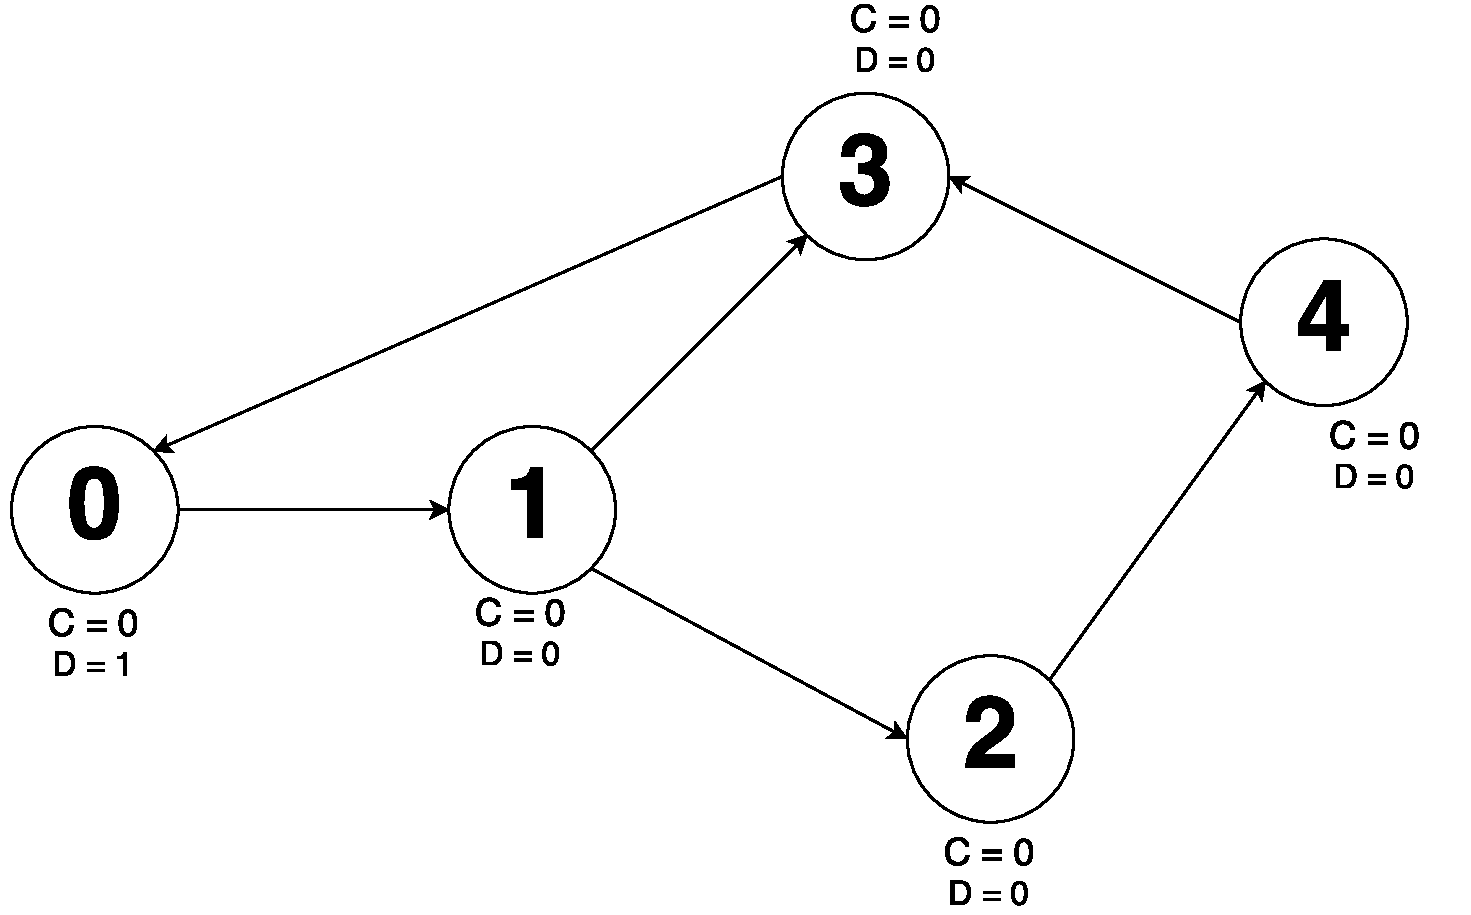
\includegraphics[width=\linewidth]{q2/1.pdf}
		\end{figure}
		\begin{figure}[H]
			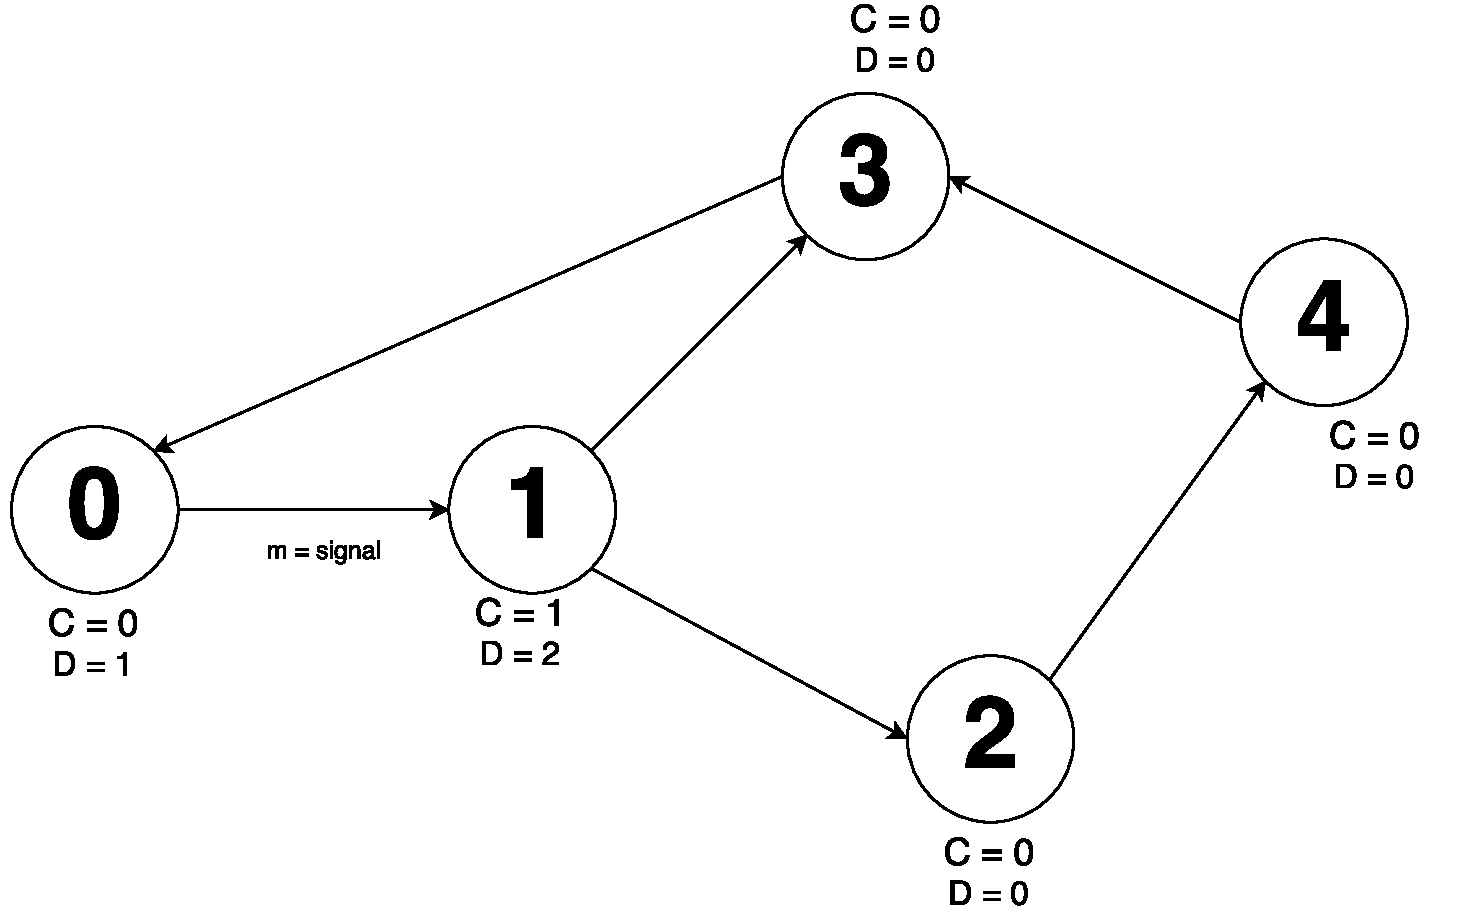
\includegraphics[width=\linewidth]{q2/2.pdf}
		\end{figure}
		\begin{figure}[H]
			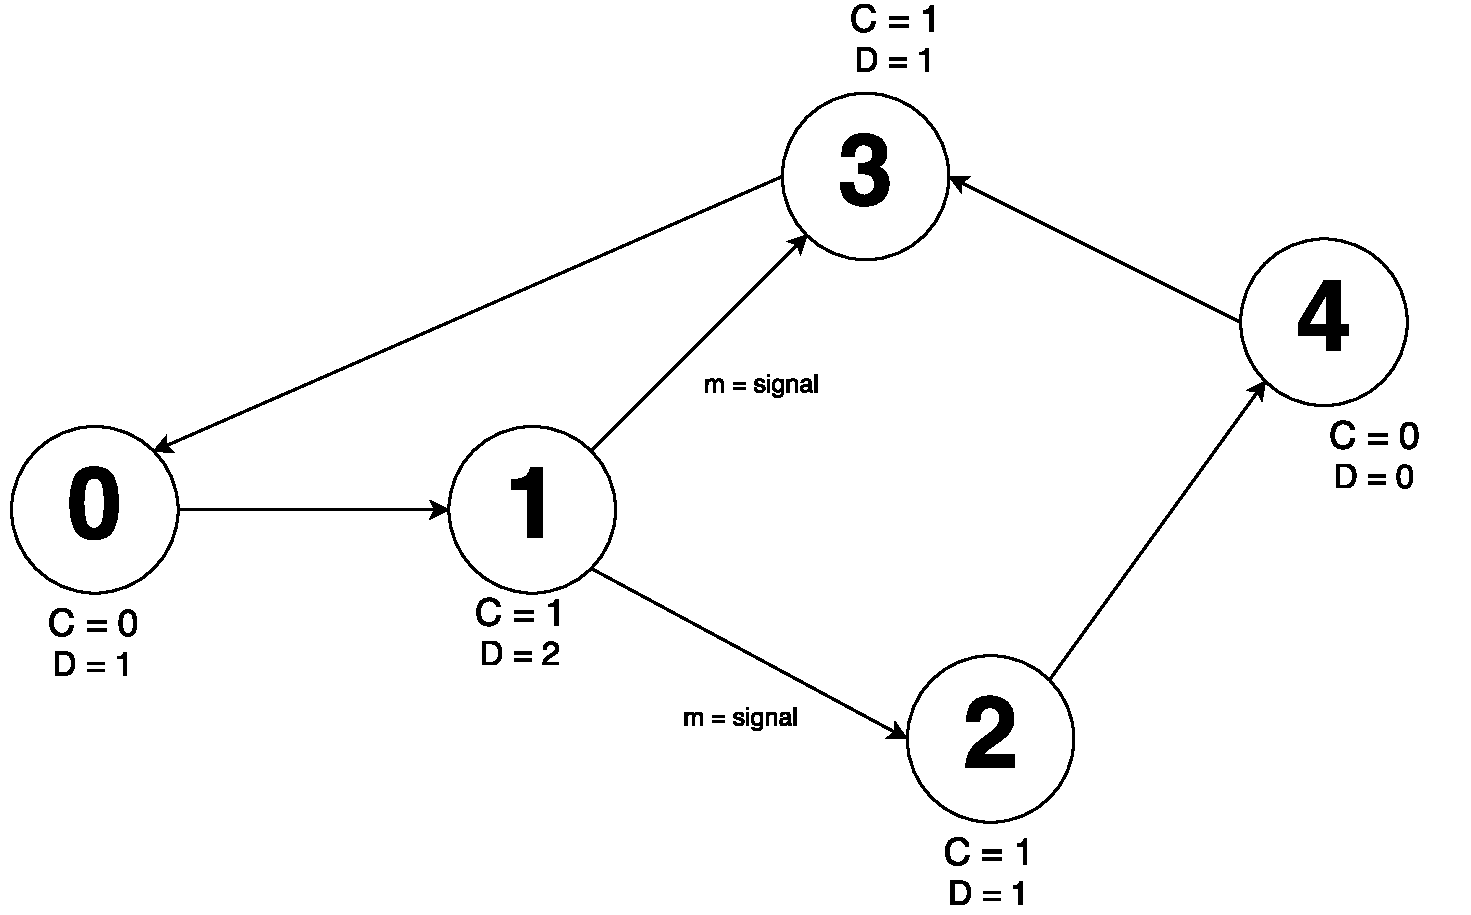
\includegraphics[width=\linewidth]{q2/3.pdf}
		\end{figure}
		\begin{figure}[H]
			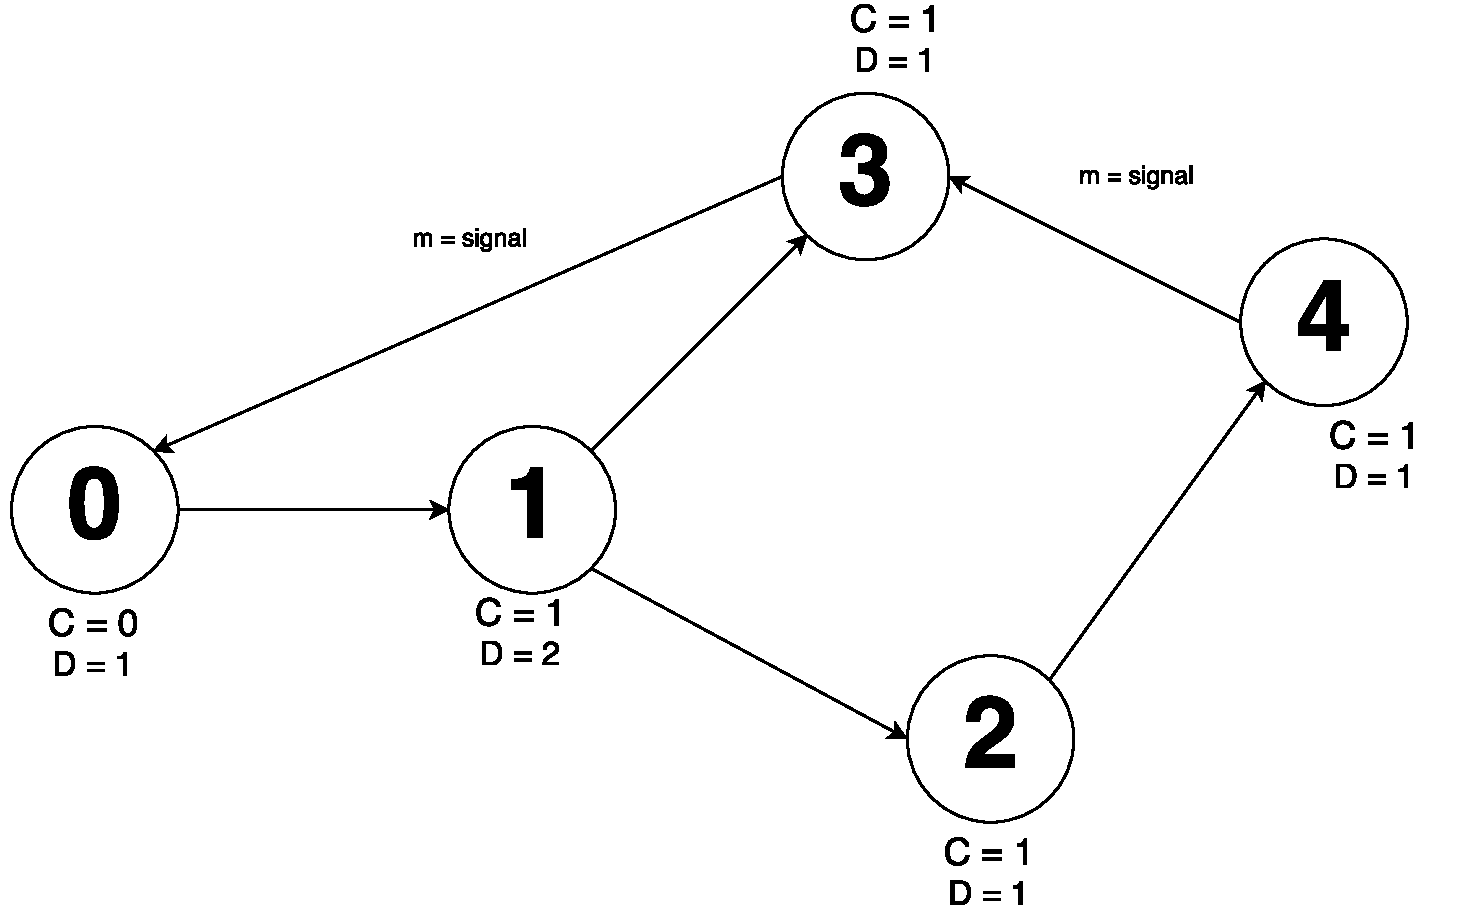
\includegraphics[width=\linewidth]{q2/4.pdf}
		\end{figure}
		\begin{figure}[H]
			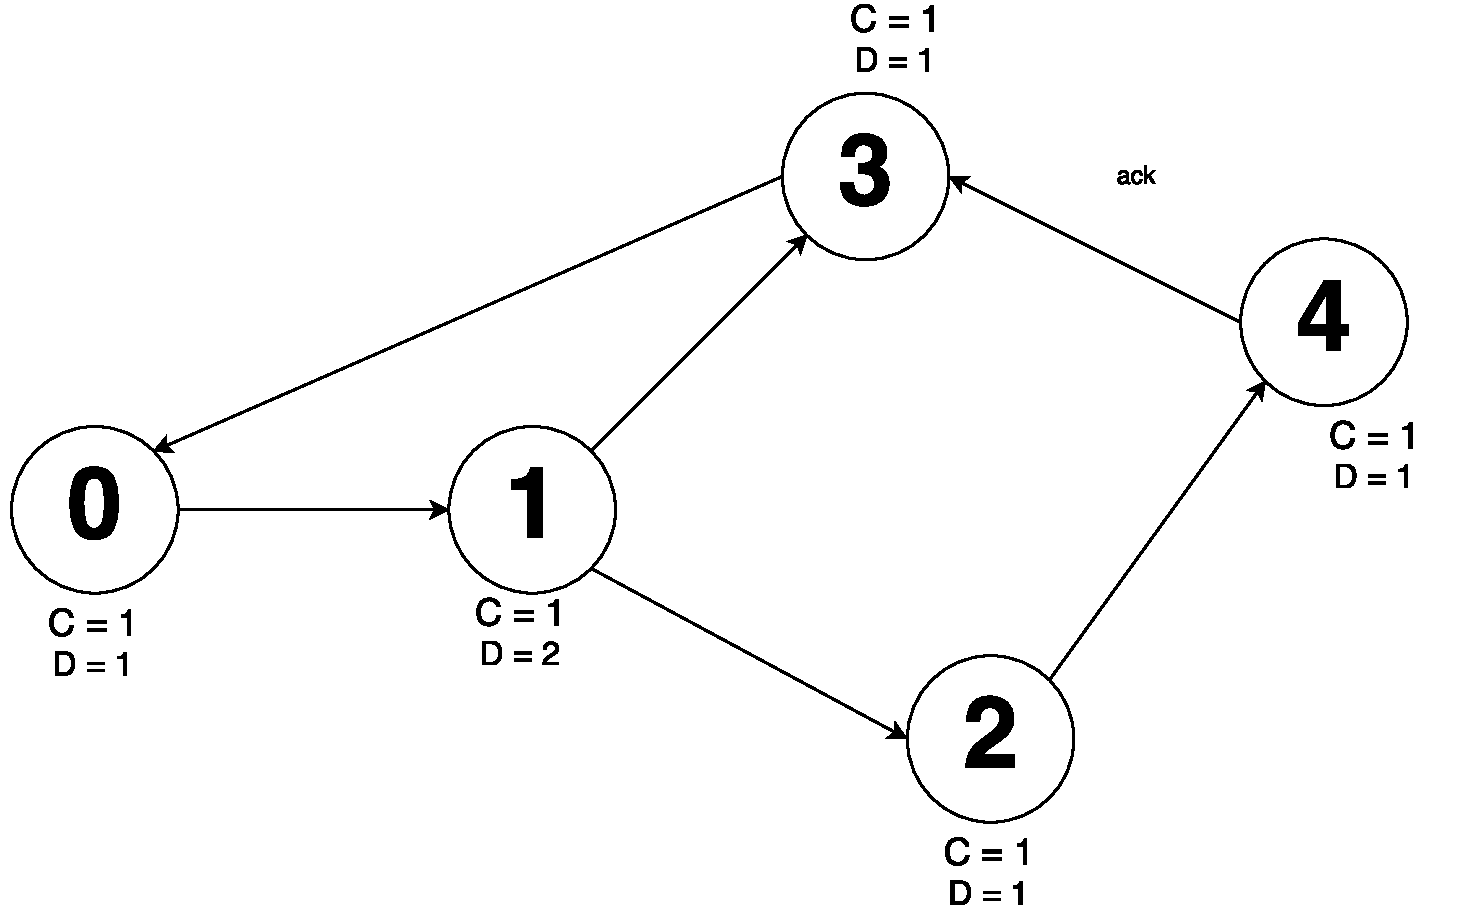
\includegraphics[width=\linewidth]{q2/5.pdf}
		\end{figure}
		\begin{figure}[H]
			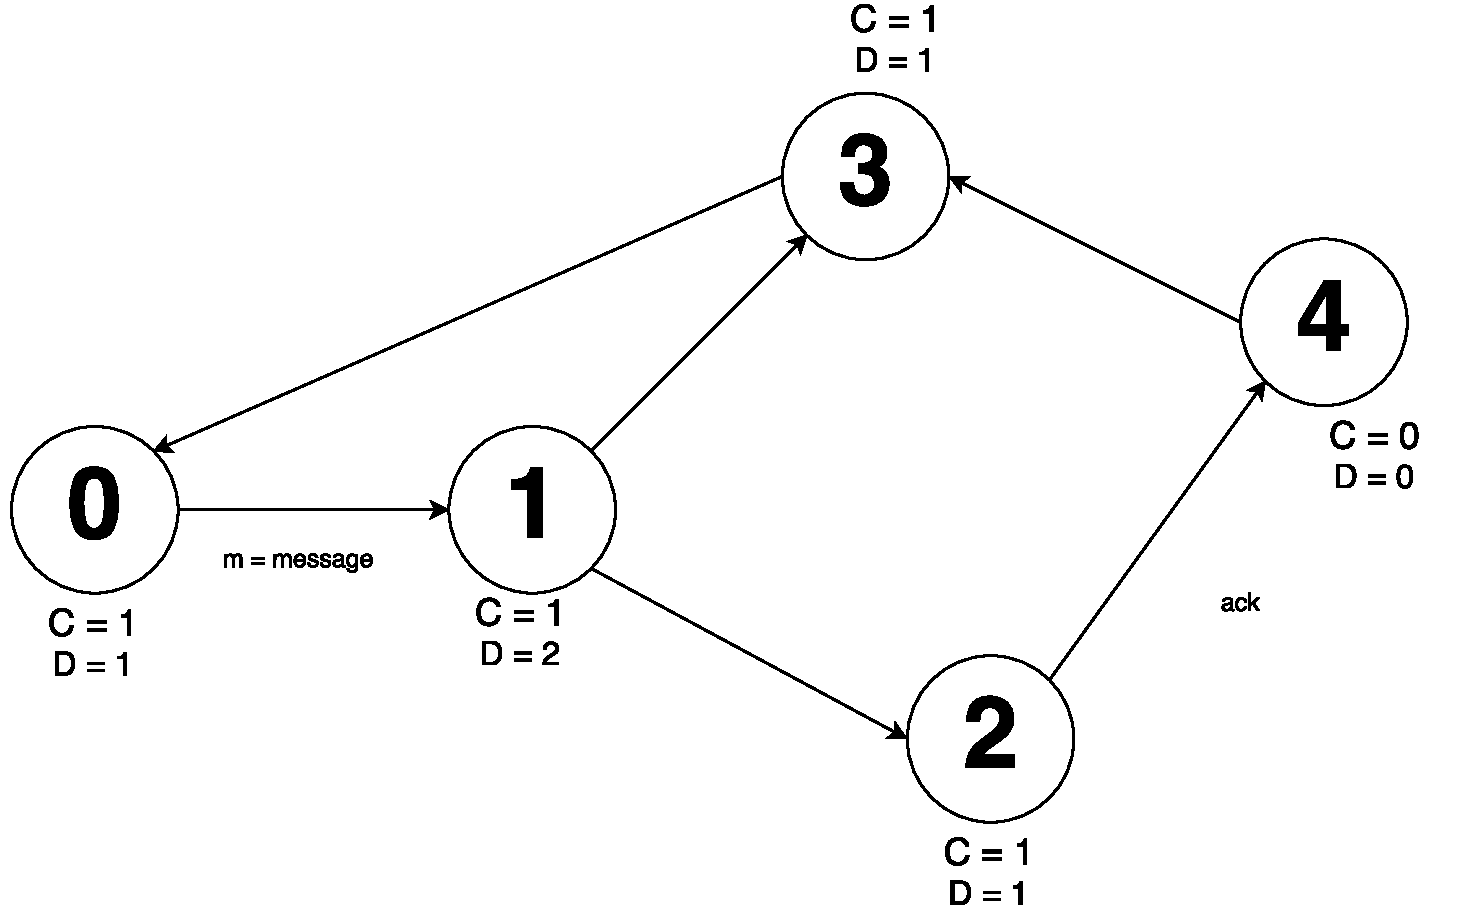
\includegraphics[width=\linewidth]{q2/6.pdf}
		\end{figure}
		\begin{figure}[H]
			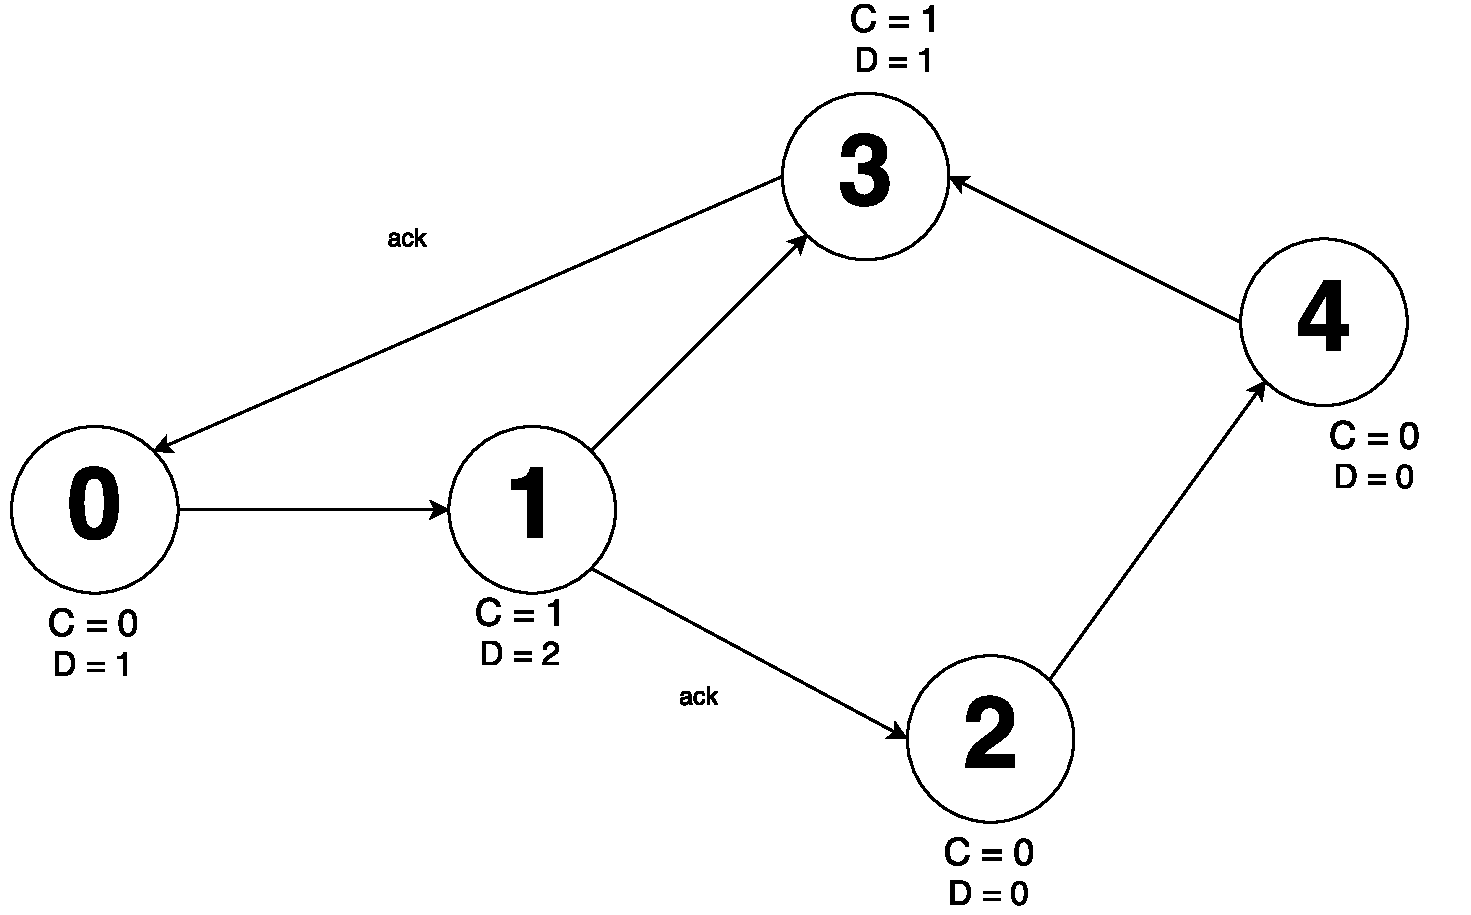
\includegraphics[width=\linewidth]{q2/7.pdf}
		\end{figure}
		\begin{figure}[H]
			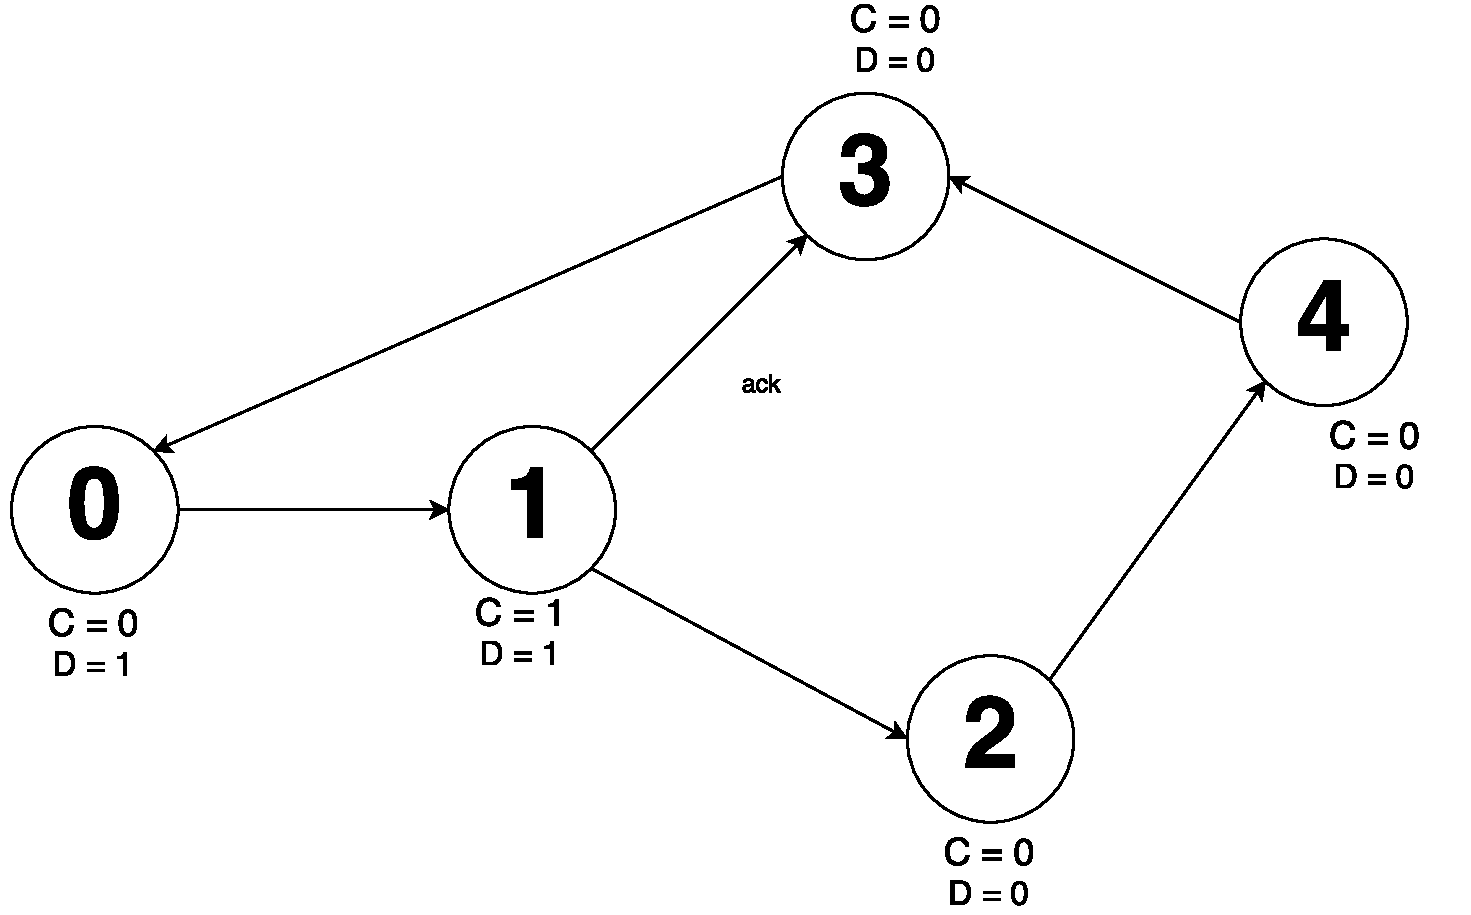
\includegraphics[width=\linewidth]{q2/8.pdf}
		\end{figure}
		\begin{figure}[H]
			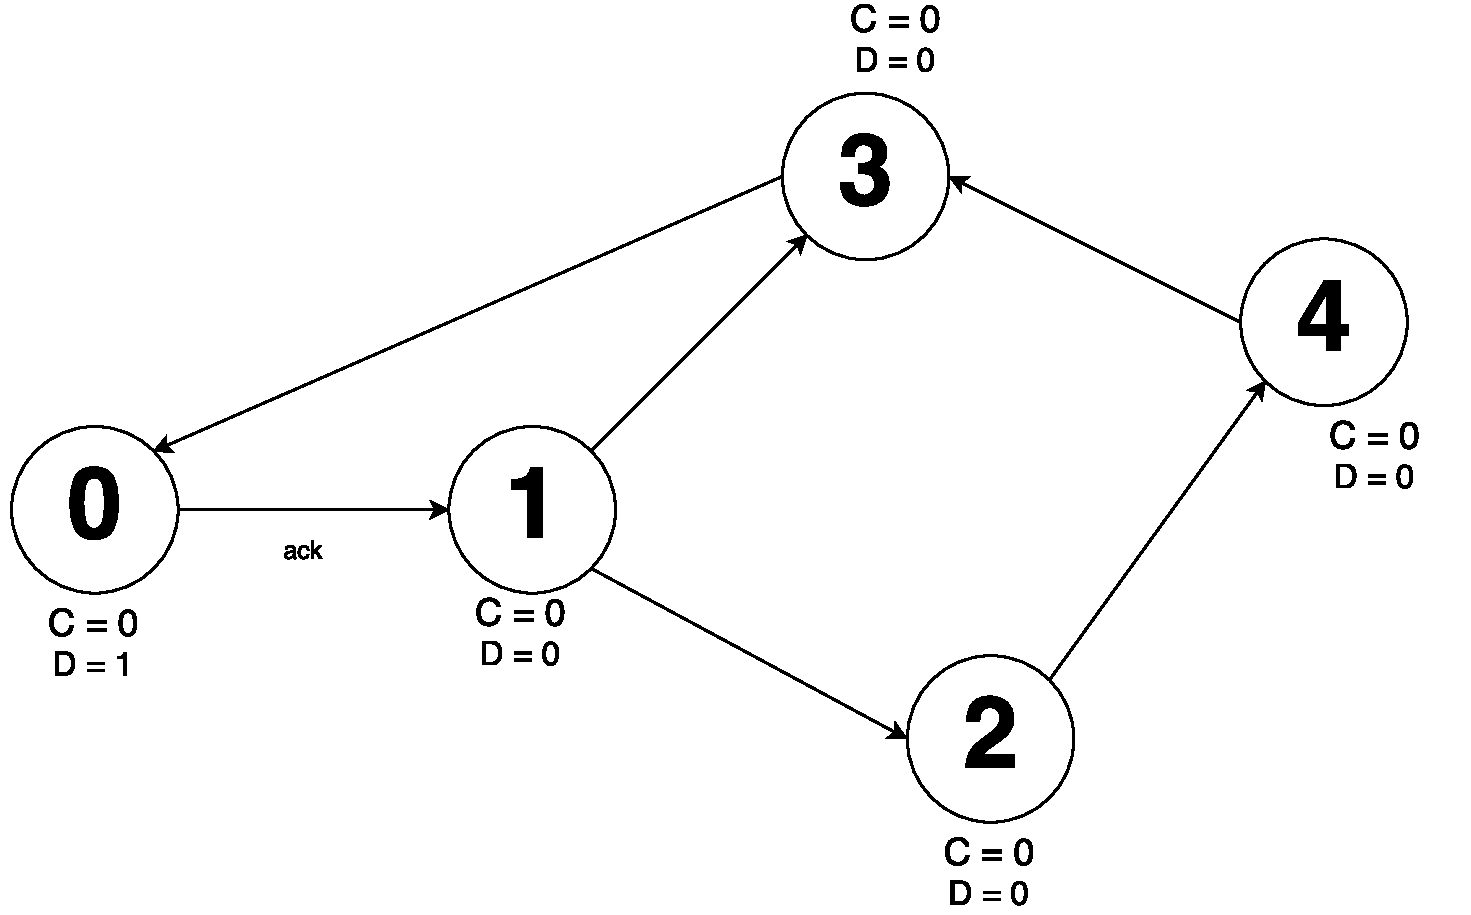
\includegraphics[width=\linewidth]{q2/9.pdf}
		\end{figure}
		\begin{figure}[H]
			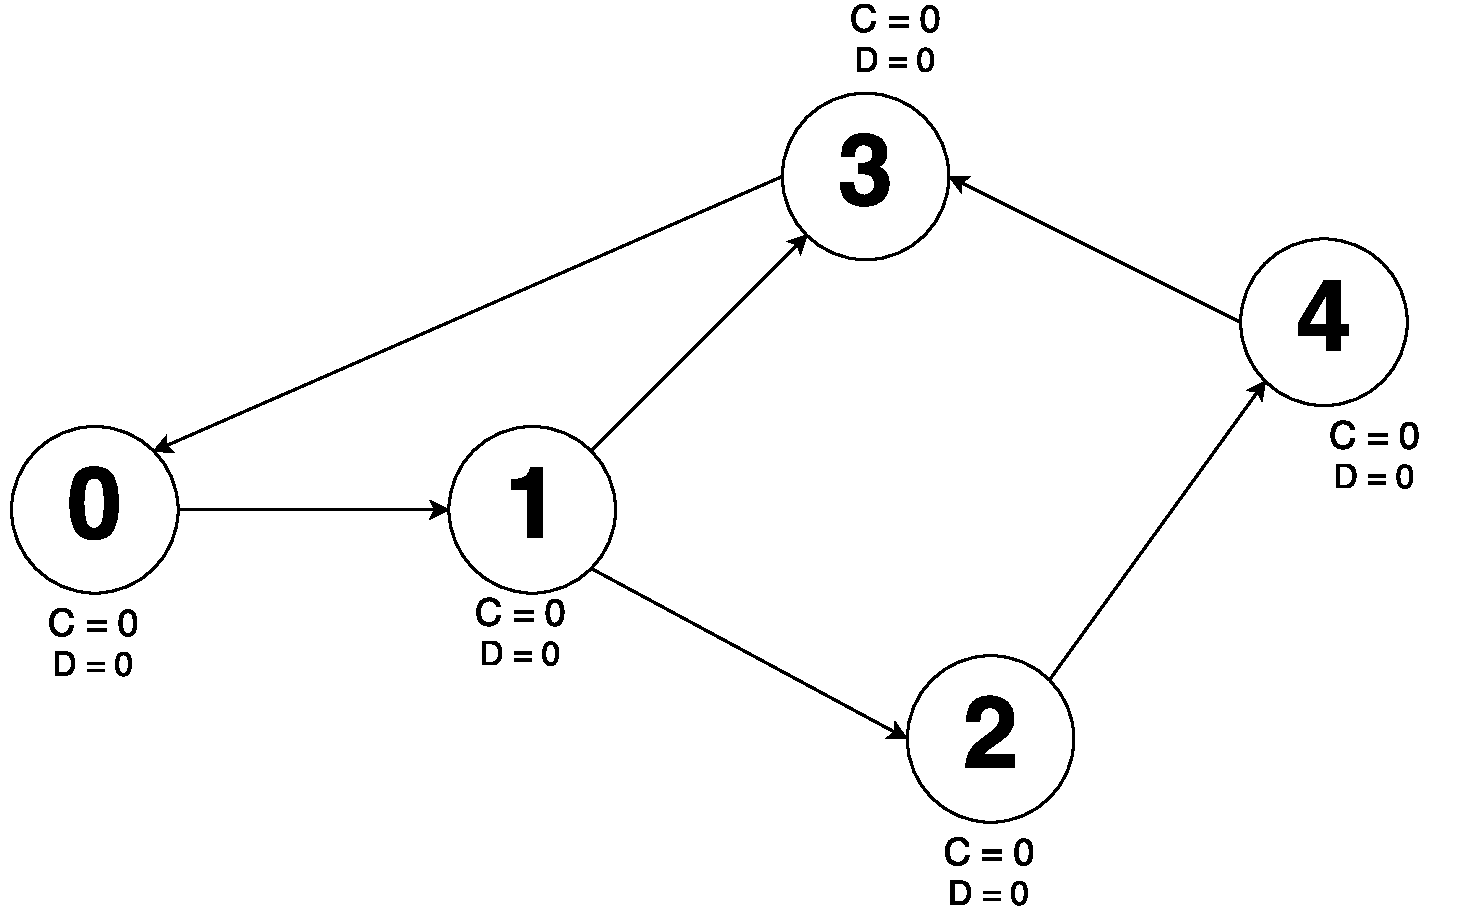
\includegraphics[width=\linewidth]{q2/10.pdf}
		\end{figure}
	\pagebreak
	%Problem 3
	\section{Define what the reliable end-to-end transmission is. Using induction, prove the Stenning protocol can achieve reliable end-to-end transmission.}
		Reliable end-to-end transmission means that there most be:
		\begin{enumerate}
			\item No loss: The receiver eventually delivers each message sent out by the sender.
			\item No duplication: The receiver delivers each message sent by the sender exactly once.
			\item No reordering: The receiver always delivers the message $m[i]$ before $m[i+1]$
		\end{enumerate}
		Proof by induction that reliable end-to-end transmission is achieved:\\
		Base Case: 0 messages are sent
		
		Since no messages are sent it is not possible for the receiver to have any lost, duplicated, or reordered. Therefore, reliable end-to-end transmission holds for the base case.\\\\
		Induction Step: assume $k$ messages have been sent with the reliable end-to-end transmission holding.\\		
		Prove reliable end-to-end transmission holds for $k+1$ messages being sent:
		
		No loss: If the receiver does not receive $m[k+1]$, then it will not send $(ack, k+1)$, which triggers a retransmission of $m[k+1]$ until one copy of $m[k+1]$ is received and delivered by the receiver.
		
		No duplication: Once the receiver delivers $m[k+1]$ where $r=k+1$, it will increment $r$ by 1 to $k+2$. If it receives $m[k+1]$ again it will not deliver it, since its sequence number, $k+1$, no longer matches $r$.
		
		No reordering: For the same reason as no duplication, the receiver always delivers $m[k+1]$ before $m[k+2]$ since it only delivers messages with a sequence number that matches $r$. And once $m[k]$ is delivered $r$ will be incremented to $k+1$, meaning that the receiver will only deliver $m[k+1]$ next.
	
	%Problem 4
	\section{In Figure 2, show all the consistent cuts that (1) include event $d$ and (2) exclude event $d$ but include event $g$.}
		\begin{figure}[H]
			\caption{Part 1, include event $d$}
			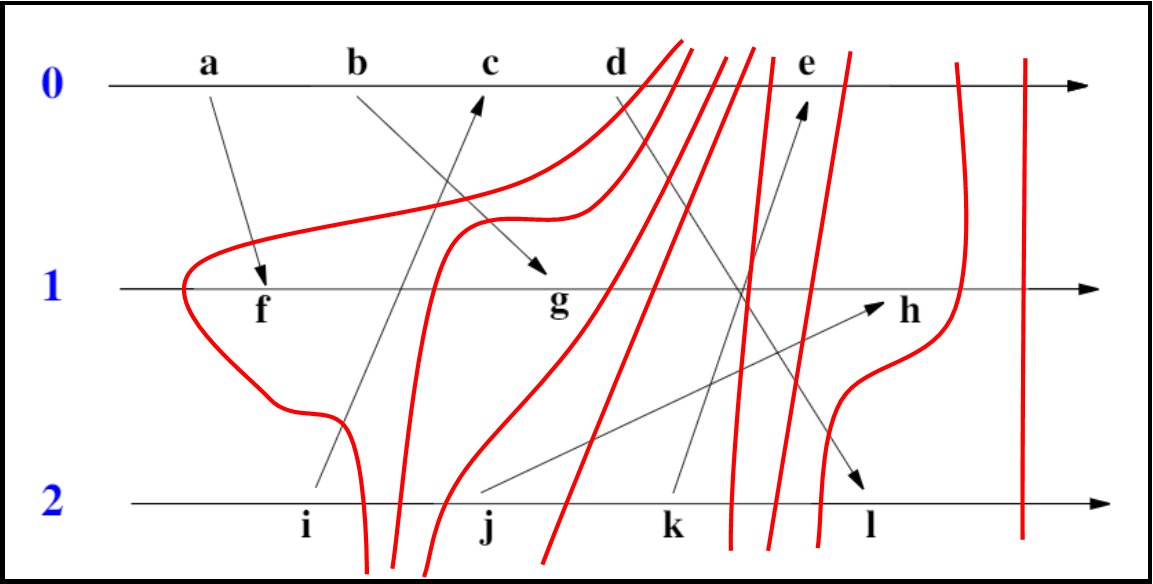
\includegraphics[width=\linewidth]{q4/q4a.png}
		\end{figure}
		\begin{figure}[H]
			\caption{Part 2, exclude event $d$ but include event $g$}
			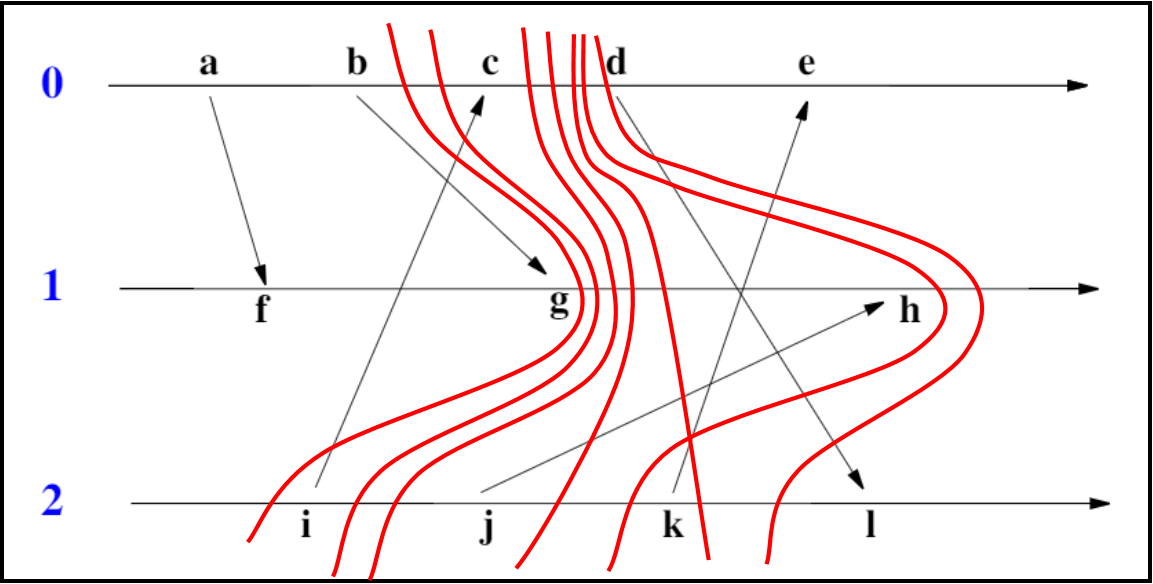
\includegraphics[width=\linewidth]{q4/q4b.png}
		\end{figure}

	\pagebreak
	%Problem 5
	\section{Assuming that any process can be the initiator, use the Chandy-Lamport algorithm to record a snapshot under the system configuration given in Figure 3, and using the recorded snapshot to compute the number of tokens in the system. Note that you can define your own local variables and the number of tokens in the system is arbitrary.}
	
	Let each process have a local variable $TokensSent=[\ ]$. Whenever a process sends a token it appends the tokens id. 
	
	At state one process 0 sends token 1 updating its local variable $TokensSent_0=[1]$, process 1 sends token 0 updating its local variable $TokensSent_1=[0]$, process 0 records its snapshot $Snapshot[0]: TokensSent_0=[1]$, and then sends the marker to process 1. 
	
	At state two process 1 sends token 1 updating its local variable $TokensSent_1=[0,1]$, process 2 sends token 0 updating its local variable $TokensSent_2=[0]$, process 1 records its snapshot $Snapshot[1]: TokensSent_1=[0,1]$, and then sends the marker to process 2. 
	
	At state three process 2 sends token 1 updating its local variable $TokensSent_2=[0,1]$, process 0 sends token 0 updating its local variable $TokensSent_0=[1,0]$, process 2 records its snapshot $Snapshot[2]: TokensSent_2=[0,1]$, and then sends the marker to process 0.
	
	At state 4 the algorithm has finished recording snapshots and the final snapshots are: $Snapshot: TokensSent_0=[1],TokensSent_1=[0,1],TokensSent_2=[0,1]$
	
	With these snapshots it can be seen by counting the number of unique token ids in $TokensSent_1$ that there are two tokens.

		\begin{figure}[H]
			\caption{State 1}
			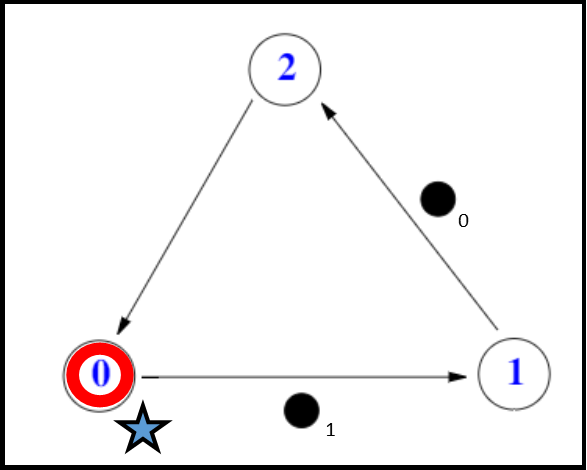
\includegraphics[width=.5\linewidth]{q5/q5a.png}
		\end{figure}
		\begin{figure}[H]
			\caption{State2}
			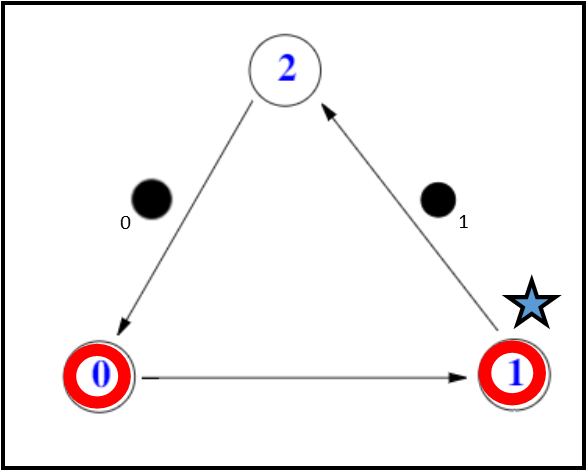
\includegraphics[width=.5\linewidth]{q5/q5b.png}
		\end{figure}
		\begin{figure}[H]
			\caption{State 3}
			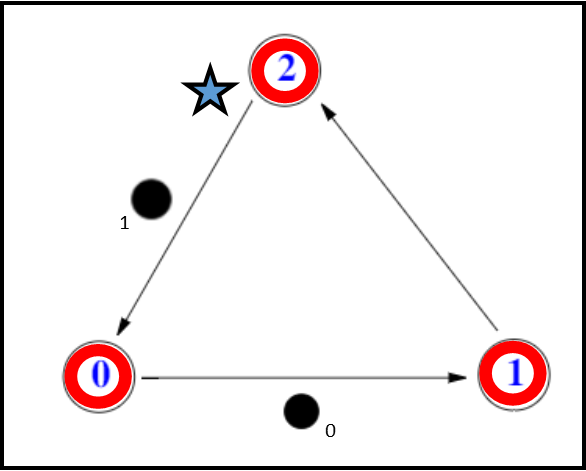
\includegraphics[width=.5\linewidth]{q5/q5c.png}
		\end{figure}
		\begin{figure}[H]
			\caption{State 4}
			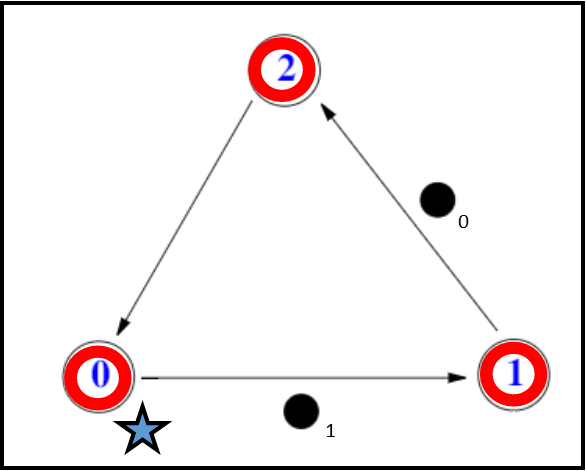
\includegraphics[width=.5\linewidth]{q5/q5d.png}
		\end{figure}

	
		
\end{document}